\documentclass{article}

% if you need to pass options to natbib, use, e.g.:
%     \PassOptionsToPackage{numbers, compress}{natbib}
% before loading neurips_2018

% ready for submission
% \usepackage{neurips_2018}

% to compile a preprint version, e.g., for submission to arXiv, add add the
% [preprint] option:
     \usepackage[preprint]{neurips_2018}

% to compile a camera-ready version, add the [final] option, e.g.:
%     \usepackage[final]{neurips_2018}

% to avoid loading the natbib package, add option nonatbib:
%     \usepackage[nonatbib]{neurips_2018}

\usepackage[utf8]{inputenc} % allow utf-8 input
\usepackage[T1]{fontenc}    % use 8-bit T1 fonts
\usepackage{hyperref}       % hyperlinks
\usepackage{url}            % simple URL typesetting
\usepackage{booktabs}       % professional-quality tables
\usepackage{amsfonts}       % blackboard math symbols
\usepackage{nicefrac}       % compact symbols for 1/2, etc.
\usepackage{microtype}      % microtypography
\usepackage{bm}
\usepackage{mathtools}
\usepackage{subcaption}
\usepackage{cleveref}
\usepackage{listings}

\newcommand{\pd}[2]{\frac{\partial #1}{\partial #2}} 

\title{Practical 1: MLPs, CNNs and Backpropagation}

% The \author macro works with any number of authors. There are two commands
% used to separate the names and addresses of multiple authors: \And and \AND.
%
% Using \And between authors leaves it to LaTeX to determine where to break the
% lines. Using \AND forces a line break at that point. So, if LaTeX puts 3 of 4
% authors names on the first line, and the last on the second line, try using
% \AND instead of \And before the third author name.

\author{%
  Erik Jenner\\
  ID 13237896
}

\begin{document}
% \nipsfinalcopy is no longer used

\maketitle

\section{MLP backprop and NumPy Implementation}
\subsection{Evaluating the Gradients}
\subsubsection{Linear Module}
Given a linear module \(\bm Y = \bm X \bm W^T + \bm B\), we want to find the gradients
of the loss with respect to \(\bm X\), \(\bm W\) and \(\bm b\).

First, we rewrite the module in index notation, using the Einstein sum convention:
\[Y_{ij} = X_{ik}W_{jk} + b_j\]
This gives us the following partial derivatives:
\begin{align*}
  \pd{Y_{ij}}{X_{mn}} &= \delta_{im}\delta_{kn}W_{jk} = \delta_{im}W_{jn}\\
  \pd{Y_{ij}}{W_{mn}} &= X_{ik}\delta_{jm}\delta_{kn} = \delta_{jm}X_{in}\\
  \pd{Y_{ij}}{b_n} &= \delta_{jn}
\end{align*}

Using the chain rule, we get
\begin{align*}
\left(\pd{L}{\bm X}\right)_{mn} &= \pd{L}{Y_{ij}} \pd{Y_{ij}}{X_{mn}} = \pd{L}{Y_{mj}}W_{jn}\\
\left(\pd{L}{\bm W}\right)_{mn} &= \pd{L}{Y_{ij}} \pd{Y_{ij}}{W_{mn}} = \pd{L}{Y_{im}}X_{in}\\
\left(\pd{L}{\bm b}\right)_n &= \pd{L}{Y_{ij}} \pd{Y_{ij}}{b_n} = \sum_{i} \pd{L}{Y_{in}}
\end{align*}
We can rewrite this in matrix form as
\begin{align*}
\pd{L}{\bm X} &= \pd{L}{\bm Y} \bm W\\
\pd{L}{\bm W} &= \left(\pd{L}{\bm Y}\right)^T \bm X\\
\pd{L}{\bm b} &= \bm 1^T \pd{L}{\bm Y}
\end{align*}
where \(\bm 1\) is the column vector of ones.

\subsubsection{Activation Module}
An activation module is given by \(Y_{ij} = h(X_{ij})\).
The derivative of an activation module is given by
\begin{align*}
  \left(\pd{L}{X}\right)_{mn} &= \pd{L}{Y_{ij}}\pd{Y_{ij}}{X_{mn}}\\
                              &= \sum_{i, j} \pd{L}{Y_{ij}}h'(X_{ij}) \delta_{im}\delta_{jn}\\
                              &= \pd{L}{Y_{mn}}h'(X_{mn}) \quad \text{(no sum)}
\end{align*}
In matrix notation, this is
\[\pd{L}{\bm X} = \pd{L}{\bm Y} \circ h'(\bm X)\]
where \(\circ\) denotes the Hadamard product and the derivative \(h'\) is applied point-wise.

For the ELU activation function
\[h(x) := \begin{cases}x, \quad x \geq 0\\ e^x - 1, \quad x < 0\end{cases}\]
this derivative is
\[h'(x) = \begin{cases}1, \quad x \geq 0\\ e^x, \quad x < 0\end{cases}\]

\subsubsection{Softmax and Loss Modules}
The softmax module is given by
\[Y_{ij} = \frac{\exp(X_{ij})}{\sum_k \exp(X_{ik})}\]
Using the quotient and chain rule, its derivative is therefore
\begin{align*}
  \pd{L}{X_{mn}} &= \sum_{i, j} \pd{L}{Y_{ij}} \pd{Y_{ij}}{X_{mn}}\\
               &= \sum_{i, j} \pd{L}{Y_{ij}} \frac{\exp(X_{ij})\delta_{im}\delta_{jn}\sum_k \exp(X_{ik})
                 - \exp(X_{ij})\sum_k \exp(X_{ik}) \delta_{im}\delta_{kn}}{\left(\sum_k \exp(X_{ik})\right)^2}\\
               &= \sum_j \pd{L}{Y_{mj}} \frac{\exp(X_{mn})\delta_{jn}\sum_k \exp(X_{mk})
                 - \exp(X_{mj})\exp(X_{mn})}{\left(\sum_k \exp(X_{mk})\right)^2}\\
               &= \pd{L}{Y_{mn}} \frac{\exp(X_{mn})}{\sum_k \exp(X_{mk})}
                 - \sum_j \pd{L}{Y_{mj}} \frac{\exp(X_{mj})\exp(X_{mn})}{\left(\sum_k \exp(X_{mk})\right)^2}\\
               &= \pd{L}{Y_{mn}} Y_{mn} - \sum_j \pd{L}{Y_{mj}} Y_{mj} Y_{mn}
\end{align*}
To avoid confusion, we've written out the sums just in this case. We never sum over \(m\) and \(n\)
even where the Einstein convention tells us to.

The categorical cross entropy loss module is given by
\[L = -\frac{1}{S}\sum_{i, k} T_{ik} \log(X_{ik})\]
where \(\bm T\) is the matrix of one-hot labels and \(S\) is the size of the batch dimension.
Since the true labels \(\bm T\) are fixed, we only need the derivative with respect to \(\bm X\):
\begin{align*}
  \pd{L}{\bm X_{mn}} &= -\frac{1}{S}\sum_{i, k} T_{ik} \frac{\delta_{im}\delta_{kn}}{X_{ik}}\\
  &= -\frac{1}{S} \frac{T_{mn}}{X_{mn}}
\end{align*}
We could write this as
\[\pd{L}{\bm X} = - \frac{1}{S} \bm T \circ \frac{1}{\bm X}\]
where \(\frac{1}{\bm X}\) is the pointwise inverse of \(\bm X\) (not \(\bm X^{-1}\)!).

\subsection{NumPy implementation}
\begin{figure}
  \centering
  \begin{subfigure}{.49\linewidth}
    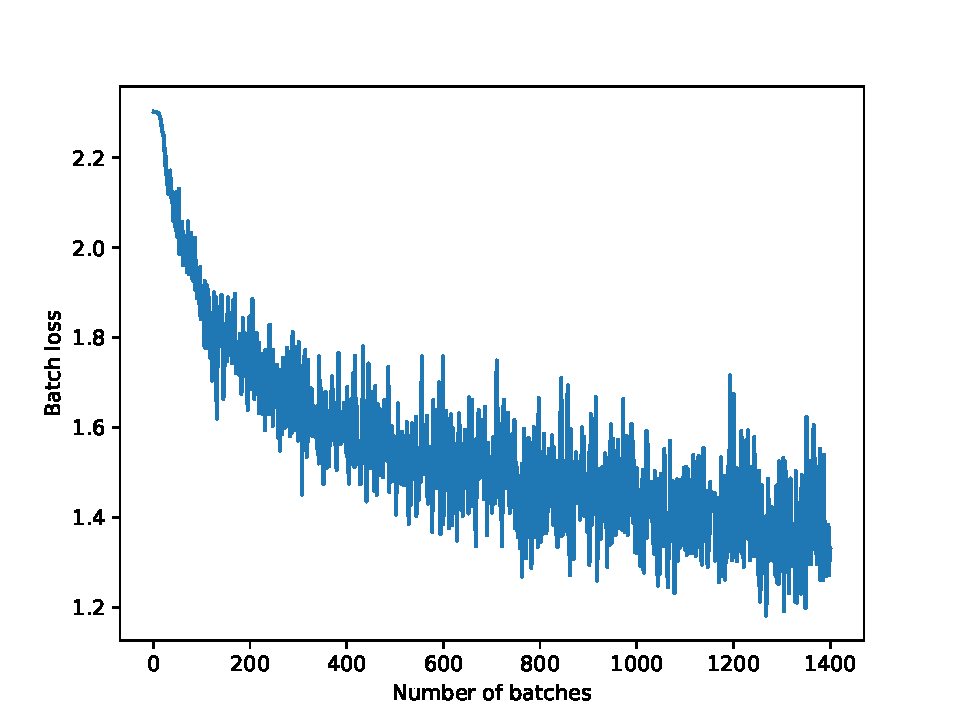
\includegraphics[width=\linewidth]{fig/np_default/loss_curve.pdf}
    \caption{Loss}
  \end{subfigure}
  \begin{subfigure}{.49\linewidth}
    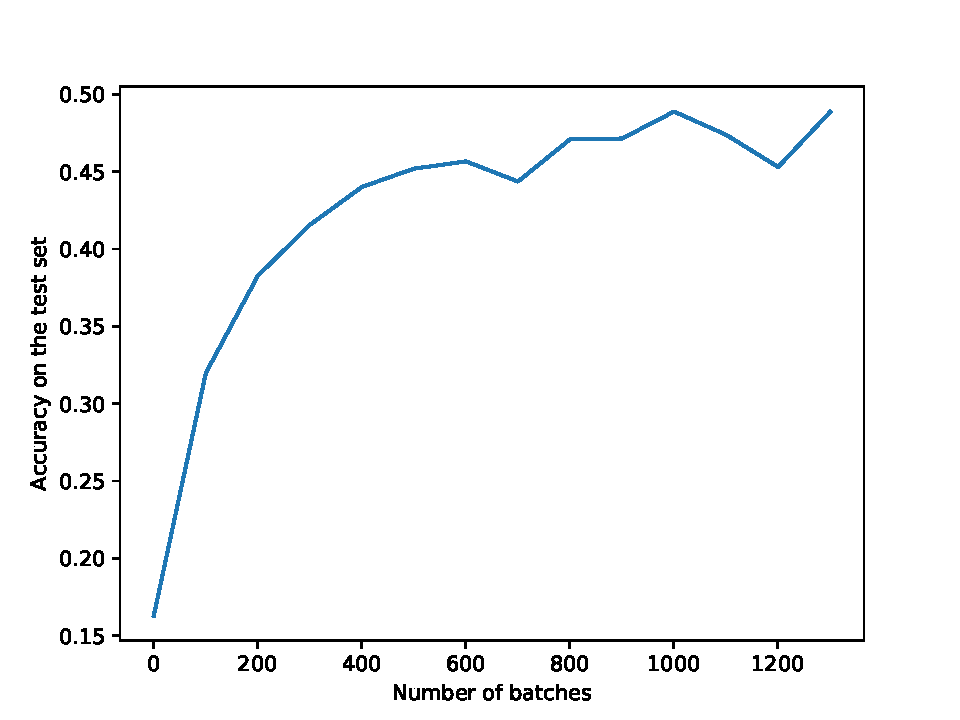
\includegraphics[width=\linewidth]{fig/np_default/accuracy_curve.pdf}
    \caption{Accuracy}
  \end{subfigure}
  \caption{Train loss and test accuracy curve with default settings}
  \label{fig:np_default}
\end{figure}

\Cref{fig:np_default} shows the loss and accuracy curves of the NumPy implementation
with default settings. The final test set accuracy after 1400 batches is 48.38\%.

\section{PyTorch MLP}
\subsection{Experiments}
With the default settings from the NumPy implementation, including the same initialization,
I get an accuracy of 49.12\%. The small difference to the NumPy version presumably comes
from different random numbers because the seeding procedures of NumPy and PyTorch are
not the same. Just increasing the number of iterations does not help significantly (the accuracy
peaks at slightly more than 50\% after 2300 steps).

To get significantly better results, I wanted to increase the number of layers. But with the default
initialization scheme (constant variance of 0.0001), two hidden layers lead to no learning at all, so I instead
normalized the input to unit variance per channel and used PyTorch's default initialization
for the linear layers.

Even so, training didn't work well and my network with two hidden layers underperformed
the baseline with default parameters. Switching the optimizer from SGD to Adam (with its default
PyTorch settings) lead to very large improvements.

With hidden layers of sizes [200, 200, 150, 100, 100] and longer training, I then reached the 52\%
accuracy. However, performance plateaued relatively early. To profit from long training times,
I introduced a learning rate scheduler that decreased the learning rate by a factor of 0.5 every 500
iterations. With these settings, I reached an accuracy of about 56\% after 2000 iterations, after which
the performance plateaus. The loss and accuracy curves for these settings are shown in
\cref{fig:pytorch}. The noise in the loss curve comes from the fact that each loss is based on only
one batch, it does not reflect actual noise in the performance on the entire train set (though that
also exists with SGD). To reproduce these results, run\\
\begin{lstlisting}[language=bash]
  $ python train_mlp_pytorch --dnn_hidden_units \
         "200,200,150,100,100" --better-init --max_steps 4000
\end{lstlisting}

\begin{figure}
  \centering
  \begin{subfigure}{.49\linewidth}
    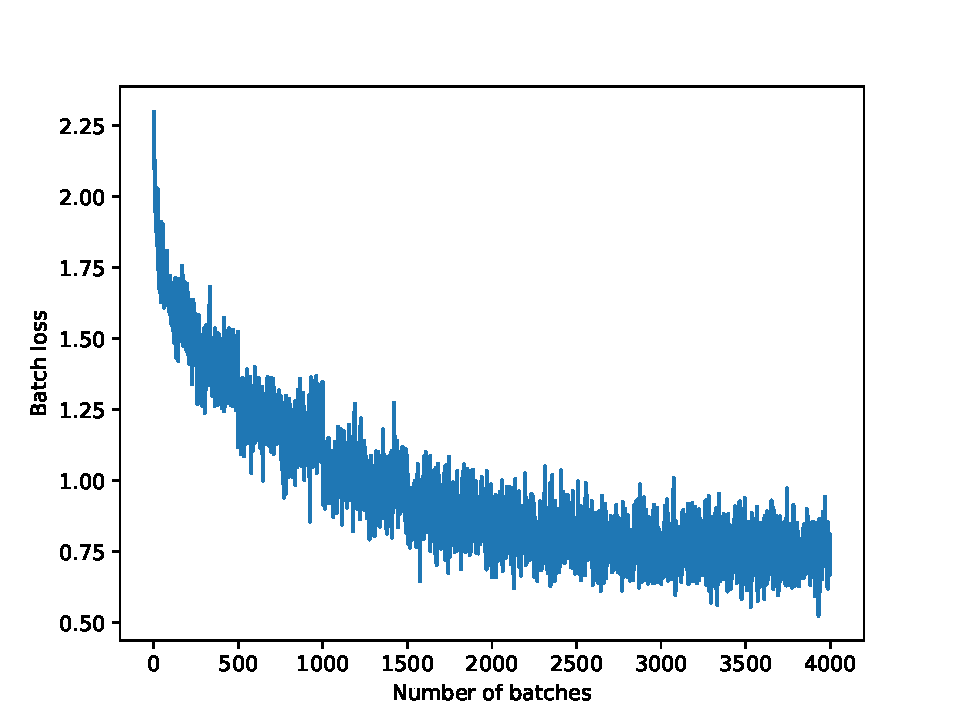
\includegraphics[width=\linewidth]{fig/pytorch_mlp/loss_curve.pdf}
    \caption{Loss}
  \end{subfigure}
  \begin{subfigure}{.49\linewidth}
    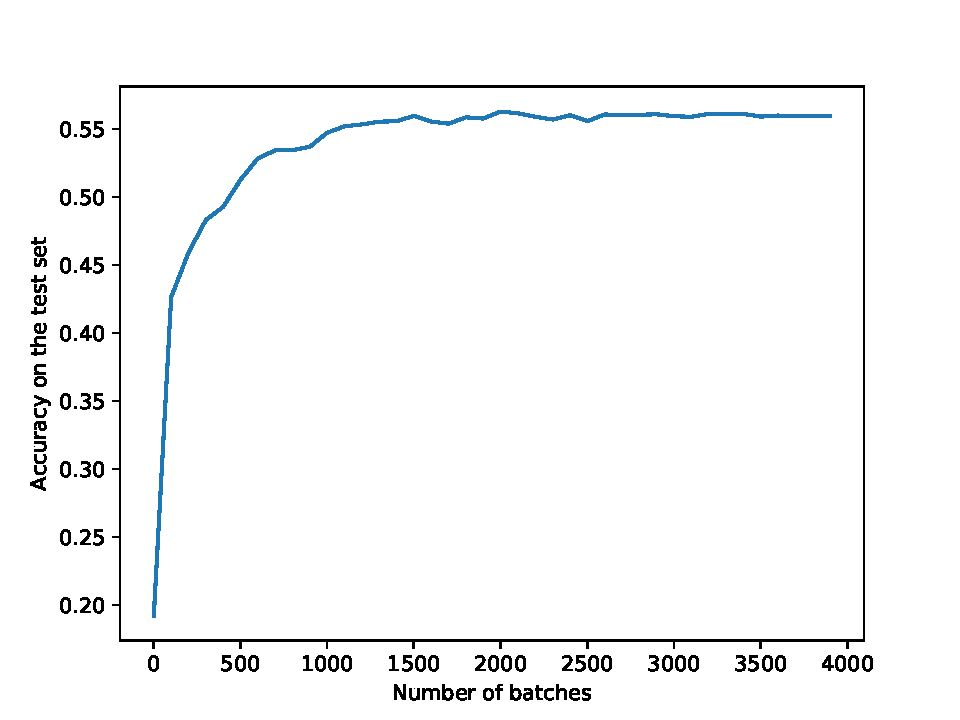
\includegraphics[width=\linewidth]{fig/pytorch_mlp/accuracy_curve.pdf}
    \caption{Accuracy}
  \end{subfigure}
  \caption{Train loss and test accuracy curve with the best found settings}
  \label{fig:pytorch}
\end{figure}

I also tried different learning rates than the default of 0.001, networks with more than 5 layers,
SGD with momentum, batchnorm, and weight decay, all without significant improvements of even with slightly worse
performance. It seems likely that some larger networks could achieve better performance
if all the other parameters were adjusted in the right way but they did not with the settings
I tried.

I also tried using ReLU and tanh activation functions instead of ELU but both were worse, ReLU
slightly and tanh by a lot.

To summarize, the key changes for better performance were:
\begin{itemize}
\item More than one hidden layer (five)
\item Adam instead of SGD
\item Learning rate scheduler
\end{itemize}
These changes did not help or were detrimental:
\begin{itemize}
\item Even more than five layers
\item Batchnorm
\item Weight decay
\item Different initial learning rates
\item Other activation functions (ReLU, tanh)
\end{itemize}

\subsection{Tanh vs ELU}
The main advantage of the ELU activation function over Tanh is that it doesn't saturate for large
activations. This means that it has large gradients for all positive activations, whereas the Tanh
gradients approaches zero quite quickly for large inputs.

A potential advantage of Tanh is that it is symmetric. If the distribution over input activations
is symmetric around 0 (e.g. Gaussian), then so is the output distribution. In particular, the
expected value of 0 is preserved. In contrast, the ELU activation distorts symmetric distributions
and it's output may have non-zero expected value even if the input is centered around zero.
To avoid a shift in the mean activations, the bias may need to be adjusted correctly -- or in other
words: if the bias is initialized to zero, the network may initially exhibit a shift in the mean activations
over different layers.

\section{Layer normalization}
In this entire section, we do \textbf{not} use the Einstein sum convention!

The layer normalization module is given by
\[Y_{si} = \gamma_i \hat{X}_{si} + \beta_i\]
where
\[\hat{X}_{si} = \frac{X_{si} - \mu_s}{\sqrt{\sigma_s^2 + \epsilon}}\]
with \(\mu_s\) the mean and \(\sigma_s^2\) the (biased) variance of \(X_{s\cdot}\).
\subsection{Implementation using autograd}
See code
\subsection{Manual implementation of backward pass}
We first calculate the derivatives of \(Y_{si}\):
\begin{align*}
\pd{Y_{si}}{\gamma_j} &= \hat{X}_{si}\delta_{ij}\\
\pd{Y_{si}}{\beta_j} &= \delta_{ij}\\
\pd{Y_{si}}{\hat{X}_{lj}} &= \gamma_i \delta_{ij}\delta_{sl}
\end{align*}

To find \(\pd{\bm Y}{\bm X}\), we first need
\begin{align*}
  \pd{\mu_s}{X_{lj}} &= \frac{1}{M}\delta_{sl}\\
  \pd{\sigma_s^2}{X_{lj}} &= \frac{1}{M}\sum_i 2(X_{si} - \mu_s) (\delta_{sl}\delta_{ij} - \pd{\mu_s}{X_{lj}})\\
                     &= \frac{2}{M}\delta_{sl} (X_{sj} - \mu_s)\\
  \pd{\hat{X}_{si}}{X_{lj}} &= \frac{(\pd{X_{si}}{X_{lj}} - \pd{\mu_s}{X_{lj}})\sqrt{\sigma_s^2 + \epsilon}
                              - (X_{si} - \mu_s) \frac{\pd{\sigma_s^2}{X_{lj}}}{2\sqrt{\sigma_s^2 + \epsilon}}}
                              {\sigma_s^2 + \epsilon}\\
                     &= \delta_{sl}\frac{\delta_{ij} - \frac{1}{M}}{\sqrt{\sigma_s^2 + \epsilon}} - \delta_{sl}\frac{1}{M}
                       \frac{(X_{si} - \mu_s)(X_{sj} - \mu_s)}{(\sigma_s^2 + \epsilon)^{3/2}}\\
  &= \frac{\delta_{sl}}{M\sqrt{\sigma_s^2 + \epsilon}}\left(M \delta_{ij} - 1 - \frac{(X_{si} - \mu_s)(X_{sj} - \mu_s)}{\sigma_s^2 + \epsilon}\right)\\
  &= \frac{\delta_{sl}}{M\sqrt{\sigma_s^2 + \epsilon}}\left(M \delta_{ij} - 1 - \hat{X}_{si}\hat{X}_{sj}\right)
\end{align*}

Now we get
\begin{align*}
  \pd{Y_{si}}{X_{lj}} &= \sum_{m, n} \pd{Y_{si}}{\hat{X}_{mn}}\pd{\hat{X}_{mn}}{X_{lj}}\\
                      &= \sum_{m, n}\gamma_i\delta_{in}\delta_{sm}\pd{\hat{X}_{mn}}{X_{lj}}\\
                      &= \gamma_i \pd{\hat{X}_{si}}{X_{lj}}\\
  &= \frac{\gamma_i \delta_{sl}}{M\sqrt{\sigma_s^2 + \epsilon}}\left(M \delta_{ij} - 1 - \hat{X}_{si}\hat{X}_{sj}\right)
\end{align*}

The derivatives of the loss are then given as follows:
\begin{align*}
  \pd{L}{\gamma_j} &= \sum_{s, i}\pd{L}{Y_{si}}\pd{Y_{si}}{\gamma_j}\\
                   &= \sum_s \pd{L}{Y_{sj}} \hat{X}_{sj}\\
  \pd{L}{\beta_j} &= \sum_{s, i}\pd{L}{Y_{si}}\pd{Y_{si}}{\beta_j}\\
                   &= \sum_s \pd{L}{Y_{sj}}\\
  \pd{L}{X_{lj}} &= \sum_{s, i}\pd{L}{Y_{si}}\pd{Y_{si}}{X_{lj}}\\
  &= \sum_i \pd{L}{Y_{li}} \frac{\gamma_i}{M\sqrt{\sigma_l^2 + \epsilon}}\left(M \delta_{ij} - 1 - \hat{X}_{li}\hat{X}_{lj}\right)
\end{align*}

\subsection{Layer normalization vs Batch normalization}
Batch normalization normalizes each feature separately over an entire batch,
with the desired mean and variance as learnable parameters. This means that
changing the weights in linear layers does not change the mean/variance
of activations, which is instead governed independently by different parameters.
This allows the network to keep the variances in a desirable range even in very
deep networks, and it allows us to use a higher learning rate because weight changes
in linear layers don't disturb the distribution of activations as much.

However, if the batch size is very small, computing the mean and variance based on
mini-batches becomes very noisy. Layer normalization works perfectly fine for
small batch sizes because it normalizes across the different features (of which there
are usually enough for statistics that are not too noisy). In contrast to batch normalization,
this does change the expressiveness of the network (the activations for all features
are forced to have the same mean/variance).

\section{Pytorch CNN}
\subsection{CNN implementation}
\begin{figure}
  \centering
  \begin{subfigure}{.49\linewidth}
    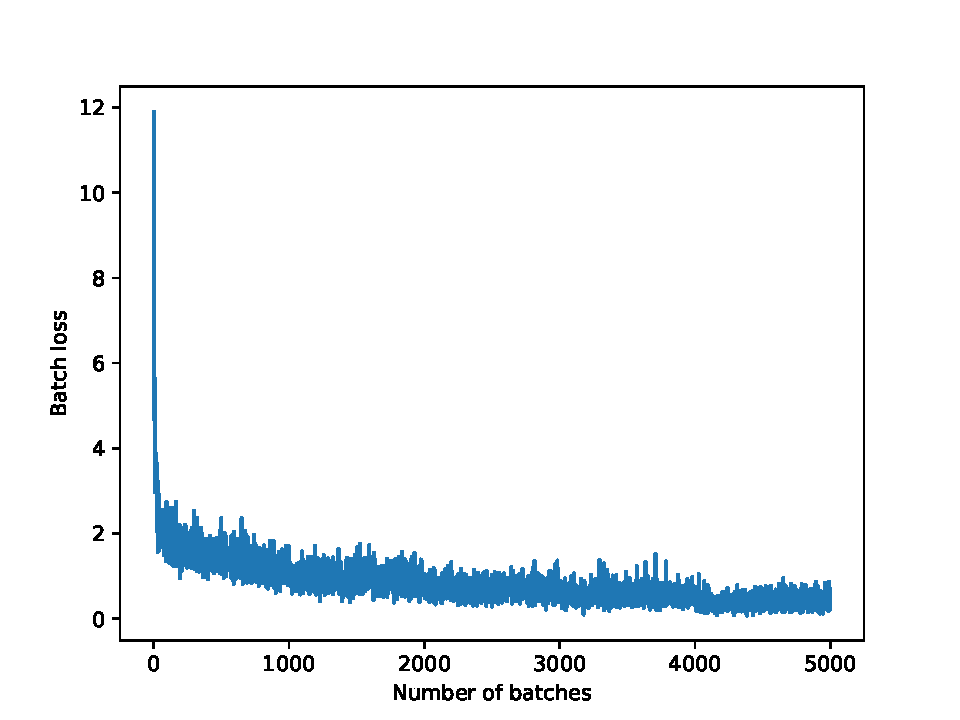
\includegraphics[width=\linewidth]{fig/cnn/loss_curve.pdf}
    \caption{Loss}
  \end{subfigure}
  \begin{subfigure}{.49\linewidth}
    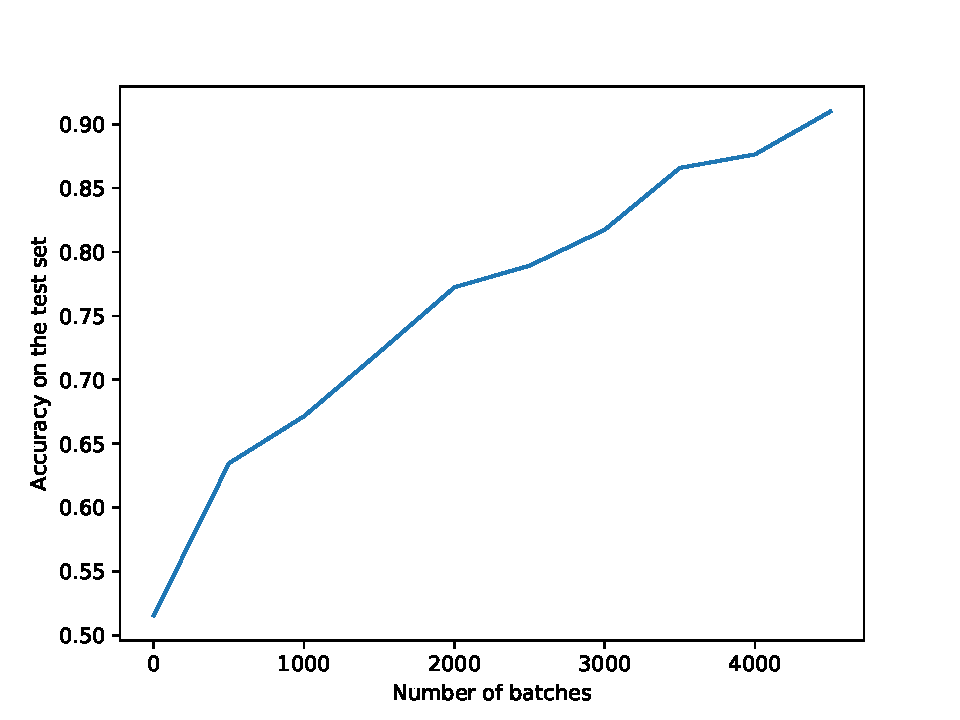
\includegraphics[width=\linewidth]{fig/cnn/accuracy_curve.pdf}
    \caption{Accuracy}
  \end{subfigure}
  \caption{Train loss and test accuracy curve with the default settings}
  \label{fig:cnn}
\end{figure}
\Cref{fig:cnn} shows loss and accuracy curves for the CNN with default settings. The test set
accuracy after 5000 batches is 91\%, better than expected from the task statement. To reproduce,
simply run \verb=$ python train_convnet_pytorch.py=.

\end{document}
%%% Local Variables:
%%% mode: latex
%%% TeX-master: t
%%% End:
